\documentclass[conference]{IEEEtran}
\IEEEoverridecommandlockouts

\usepackage{cite}
\usepackage{amsmath,amssymb,amsfonts}
\usepackage{algorithmic}
\usepackage{graphicx}
\usepackage{textcomp}
\usepackage{xcolor}
\usepackage{booktabs}
\usepackage{url}
\usepackage{microtype}
\usepackage{tabularx}

\def\BibTeX{{\rm B\kern-.05em{\sc i\kern-.025em b}\kern-.08em
    T\kern-.1667em\lower.7ex\hbox{E}\kern-.125emX}}

\begin{document}

\title{CuraCascade: An Integrated Framework for Gene--Disease Evidence Aggregation, Validation, and Research-Oriented Analysis}

\author{\IEEEauthorblockN{Udit Shokeen (Reg. No: 23BCB0001)}
\IEEEauthorblockA{\textit{School of Computer Science and Engineering} \\
\textit{Vellore Institute of Technology}\\
Vellore, Tamil Nadu 632014, India \\
Email: udit.shokeen2023@vitstudent.ac.in}
}

\maketitle

\begin{abstract}
Clinical genomics relies on expert consortia---most prominently the Clinical Genome Resource (ClinGen)---to establish the clinical validity of gene--disease associations. However, when expert panels re-evaluate and subsequently downgrade an association from \textit{Definitive} or \textit{Moderate} validity to \textit{Limited} (insufficient evidence), \textit{Disputed} (conflicting evidence), or \textit{Refuted} (evidence against validity), downstream repositories do not automatically synchronize. Active diagnostic assertions, including Pathogenic and Likely Pathogenic (P/LP) variant interpretations in NCBI ClinVar and diagnostic-grade (``Green'') panel indications in Genomics England PanelApp, routinely persist across static archives. Rather than rendering all variants biologically invalid across all phenotypes, these discordant entries represent potential disease-specific discrepancies requiring expert genetic review. To address this asynchronous lag, we present \textbf{CuraCascade}, an open-source clinical genomics relational audit warehouse and evidence harmonization platform. CuraCascade normalizes disparate assertions across ClinGen, ClinVar, PanelApp, and gnomAD into a Third Normal Form (3NF) relational architecture backed by transactional SQLite and analytical DuckDB engines, referencing the Mondo Disease Ontology for concept reconciliation. The framework implements a deterministic, disease-aware discrepancy classification taxonomy that accounts for allelic pleiotropy, canonical ontology crosswalks (MONDO, OMIM), and distinct disorder exclusions. Evaluated against an independently curated benchmark ($N = 100$ gene--disease validity assertions; 54 published downgrades, 46 definitive disease controls), 94 of 100 cases were evaluable and six were designated \texttt{NOT\_EVALUABLE} due to absent snapshot records. Across this primary evaluable cohort ($N = 94$), CuraCascade achieved a precision of 100.0\% (95\% Wilson CI: 82.4\%--100.0\%; 18 True Positives, 0 False Positives), recall of 34.6\% (95\% CI: 23.2\%--48.2\%; 34 False Negatives), specificity of 100.0\% (95\% CI: 91.6\%--100.0\%; 42 True Negatives), accuracy of 63.8\% (95\% CI: 53.8\%--72.8\%), and concordance $\kappa = 0.3212$. In an unadjusted 100-case sensitivity analysis assuming all six unobserved cases are unflagged non-detections, recall was 33.3\% and accuracy was 64.0\%. The low recall of 34.6\% is empirically driven by absent downstream laboratory assertions (15 cases), uningested panel curations (3 cases), and strict cross-disease phenotype boundaries (16 cases). In an empirical cross-sectional latency analysis of 51,007 active ClinVar assertions across 536 curated genes, the median elapsed discordance duration since ClinGen appraisal was 2.82 years (1,030 days; IQR: 2.98 years / 1,087 days). Retrospective exploratory machine learning yielded an AUROC of 0.857 and Brier score of 0.1508; prospective claims remain disabled pending longitudinal pre-curation feature reconstruction. CuraCascade provides an automated, vendor-neutral research audit framework to prioritize potential disease-specific discrepancies for clinical and genetic review.
\end{abstract}

\begin{IEEEkeywords}
Clinical genomics, gene curation, ClinGen, ClinVar, PanelApp, data warehouse, Third Normal Form, evidence downgrade, biomedical informatics.
\end{IEEEkeywords}

\section{Introduction}
The integration of high-throughput next-generation sequencing (NGS) into diagnostic medicine has accelerated the identification of putative monogenic disease genes. However, the clinical utility of comprehensive genomic sequencing depends fundamentally upon the veracity of the underlying gene--disease evidence base \cite{strande2017evaluating}. Historically, hundreds of monogenic disease associations were published based on candidate-gene studies involving small kindreds, inadequate statistical power, and absent ancestry-matched population control cohorts \cite{richards2015standards}. 

To establish rigorous evidence-based standardization, the Clinical Genome Resource (ClinGen) developed a semi-quantitative framework to classify gene--disease clinical validity into distinct qualitative tiers: \textit{Definitive}, \textit{Strong}, \textit{Moderate}, \textit{Limited}, \textit{Disputed}, or \textit{Refuted} \cite{strande2017evaluating, rehm2015clingen}. These classifications represent qualitatively different evidence states: \textit{Limited} denotes insufficient or preliminary evidence where clinical utility cannot yet be confirmed; \textit{Disputed} denotes conflicting evidence where substantial findings challenge the asserted causality; and \textit{Refuted} indicates affirmative evidence against the gene--disease relationship based on population genetics or contradictory pedigree segregation. Systematic reappraisals conducted by ClinGen Gene Curation Expert Panels (GCEPs) have demonstrated that up to 40\% of genes historically tested on commercial and academic panels for inherited cardiomyopathies \cite{kelly2018adaptation, ingles2019evaluating}, Brugada syndrome \cite{hosseini2018reappraisal}, and hereditary cancer \cite{lee2019clinical} lack sufficient scientific validity.

Despite formal consortium consensus updates, biomedical knowledge bases operate in decentralized, asynchronous silos. When ClinGen formally publishes a gene--disease downgrade, downstream knowledge bases---including the National Center for Biotechnology Information (NCBI) ClinVar archive \cite{landrum2020clinvar} and Genomics England PanelApp \cite{martin2019panelapp}---do not automatically propagate these re-appraisals. Consequently, variants located within disputed or refuted disease genes frequently remain cataloged as Pathogenic (P) or Likely Pathogenic (LP) in ClinVar. Similarly, diagnostic exome panels routinely retain downgraded genes as ``Green'' (diagnostic-grade), prompting clinical interpretation and reporting \cite{wright2015genetic}.

Importantly, a gene-level downgrade does not imply that all constituent variants are biologically benign across all possible phenotypes; rather, variant assertions submitted under a questioned or refuted indication represent potential disease-specific discrepancies requiring expert genetic review. If left unreviewed, reporting such variants under outdated indications can introduce diagnostic friction, misdirected clinical workups, or unwarranted familial cascade testing \cite{ingles2019evaluating}.

To address this knowledge cascade lag, we present \textbf{CuraCascade}, an integrated computational framework for gene--disease evidence aggregation, relational validation, and research-oriented discrepancy auditing.

\section{Background and Related Work}
Evidence curation in clinical genetics has evolved from individual laboratory assertions toward structured expert consensus. ClinGen GCEPs conduct systematic literature reappraisals to evaluate genetic and experimental evidence \cite{strande2017evaluating}. Concurrently, NCBI ClinVar aggregates variant-level clinical interpretations submitted by hundreds of testing laboratories worldwide \cite{landrum2020clinvar}. Genomics England PanelApp crowd-sources expert evaluations to establish diagnostic panel indications for the UK National Health Service (NHS) Genomic Medicine Service \cite{martin2019panelapp}.

Prior studies have highlighted discrepancies between variant interpretations across submitters in ClinVar \cite{richards2015standards}. However, existing quality-assurance tools focus primarily on variant-level discordance (e.g., conflicting classifications between Benign and Pathogenic) or population allele frequency ceilings via the Genome Aggregation Database (gnomAD) \cite{karczewski2020mutational}. 

Significantly less attention has been directed toward the systemic disconnect between \textit{gene-level validity reappraisals} and \textit{downstream variant-level assertions}. When an entire gene is refuted or placed in a limited-evidence tier for a specific condition, constituent variants submitted under that indication require systematic re-evaluation. Currently, diagnostic laboratories and curation teams lack automated, open-source relational infrastructure to identify, track, and prioritize these unpropagated consensus shifts for expert re-adjudication.

\section{Problem Statement and Objectives}
\subsection{Problem Statement}
Let a clinical validity assertion be a tuple $A_{\text{CG}} = (G, D, C, t_{\text{CG}})$, where $G$ is the HGNC gene symbol, $D$ is the disease concept, $C \in \{\text{Definitive}, \text{Strong}, \text{Moderate}, \text{Limited}, \text{Disputed}, \text{Refuted}\}$ is the ClinGen validity status, and $t_{\text{CG}}$ is the appraisal date. Let downstream assertions be $A_{\text{CV}} = (v, G, D', S_{\text{CV}}, t_{\text{CV}})$ for ClinVar variants and $A_{\text{PA}} = (G, D'', T_{\text{PA}})$ for PanelApp panel indications, where $S_{\text{CV}} \in \{\text{P}, \text{LP}, \text{VUS}, \text{LB}, \text{B}\}$ and $T_{\text{PA}} \in \{\text{Green}, \text{Amber}, \text{Red}\}$.

When $C \in \{\text{Limited}, \text{Disputed}, \text{Refuted}\}$ for disease $D$, an evidence discordance exists if downstream registries retain active pathogenic assertions ($S_{\text{CV}} \in \{\text{P}, \text{LP}\}$ or $T_{\text{PA}} = \text{Green}$) for a matching disease concept ($D \approx D'$). The cross-sectional elapsed latency is defined as:
\begin{equation}
\Delta t = t_{\text{obs}} - t_{\text{CG}}
\end{equation}
representing the elapsed duration during which potentially discordant diagnostic assertions remain active in operational repository circulation without expert re-adjudication.

\subsection{System Objectives}
CuraCascade was engineered to achieve four core objectives:
\begin{enumerate}
    \item \textbf{Relational Evidence Harmonization:} Ingest and harmonize multi-source assertions into a normalized Third Normal Form (3NF) relational warehouse.
    \item \textbf{Deterministic Biological Audit Engine:} Implement disease-aware matching rules that distinguish potential discrepancies from distinct disorders in pleiotropic genes.
    \item \textbf{Empirical Latency Characterization:} Quantify the empirical cross-sectional elapsed duration of active assertions across clinical specialties and submitter review tiers.
    \item \textbf{Transparent Independent Benchmarking:} Evaluate audit decision rules against an independently curated ground truth with explicit confidence intervals, stated sensitivity assumptions, and failure-mode analysis.
\end{enumerate}

\begin{figure}[t]
\centering
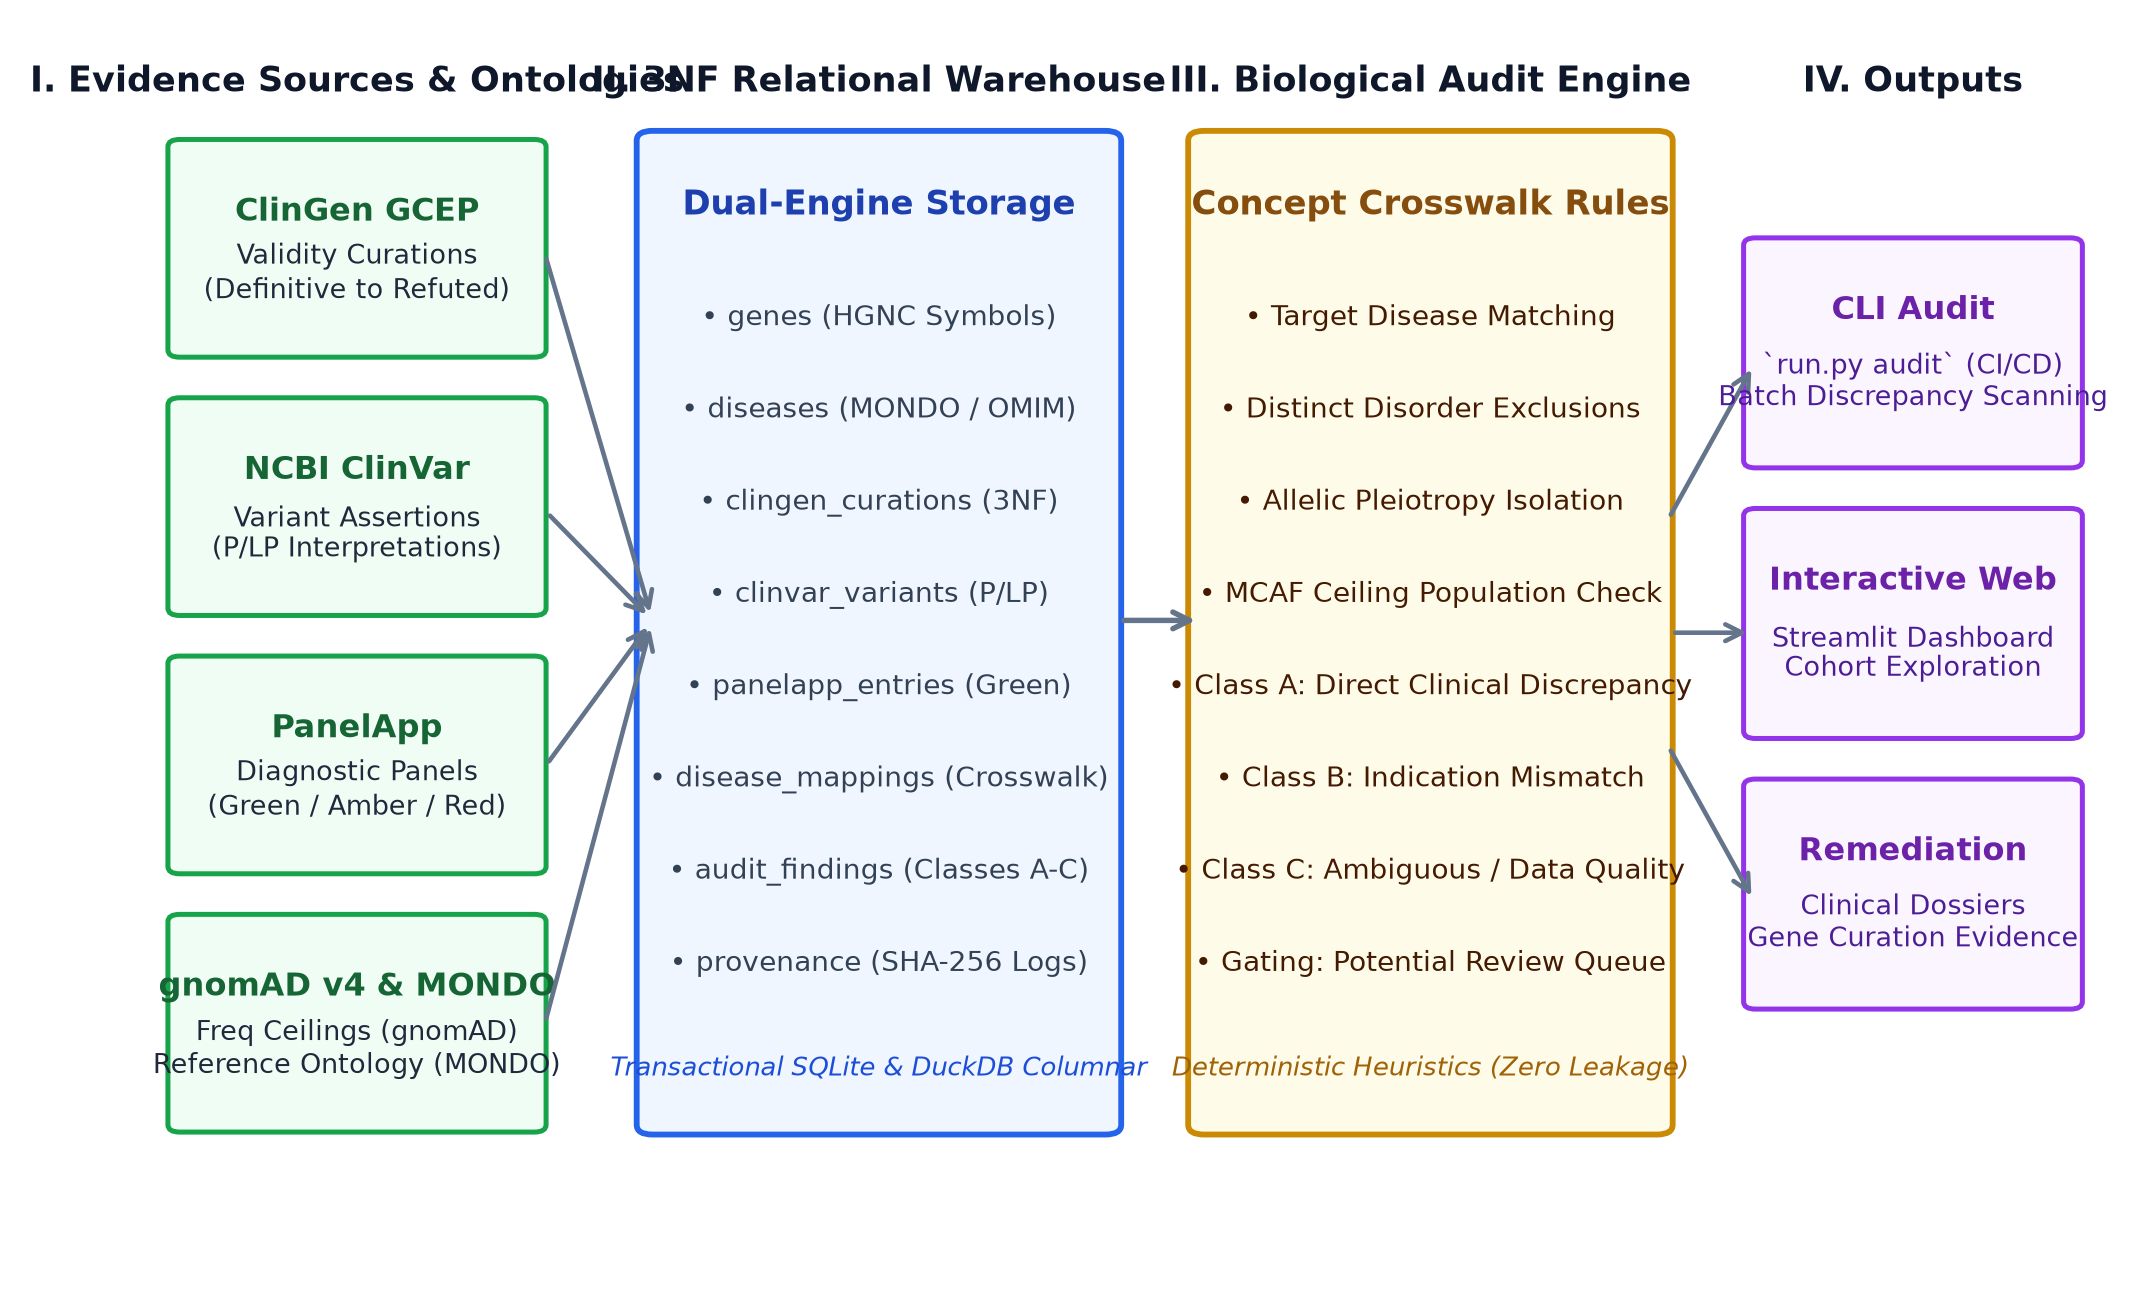
\includegraphics[width=\columnwidth]{figures/fig1_architecture.png}
\caption{Overall CuraCascade system architecture and multi-tier data flow. Primary evidence sources (ClinGen, ClinVar, PanelApp, gnomAD) and reference ontologies (MONDO) are harmonized into a 3NF relational warehouse backed by SQLite and DuckDB, evaluated by a deterministic biological audit engine, and surfaced via CLI, Web, and Remediation tools.}
\label{fig:architecture}
\end{figure}

\section{System Architecture and Methodology}
The overall architecture of CuraCascade is illustrated in Fig.~\ref{fig:architecture}. The platform comprises four integrated tiers:
\begin{enumerate}
    \item \textbf{Data Ingestion \& Normalization Layer:} Automated parsers extract gene curations from ClinGen JSON/CSV endpoints, stream-filter ClinVar variant summary archives, fetch PanelApp panel indications, and calculate gnomAD maximum credible population allele frequency (MCAF) thresholds.
    \item \textbf{3NF Relational Warehouse Layer:} Dual-engine storage combining transactional SQLite with strict foreign keys and in-memory columnar DuckDB analytical scanners \cite{raasveldt2019duckdb}.
    \item \textbf{Biological Audit \& Crosswalk Engine:} Deterministic heuristic classifier evaluating target disease ontology identifiers (MONDO, OMIM), pleiotropic exclusions, and population frequency ceilings.
    \item \textbf{Audit Interfaces \& Governance Layer:} Headless command-line interface (\texttt{run.py audit}, \texttt{run.py verify}), Streamlit web portal, and automated clinical remediation dossier generators.
\end{enumerate}

\section{Data Sources and Data Processing}
CuraCascade integrates four primary biological evidence sources alongside reference disease ontologies, summarized in Table~\ref{tab:sources}:
\begin{itemize}
    \item \textbf{ClinGen Gene Validity Archive:} Evaluates expert validity classifications. Curations classified as \textit{Limited} (insufficient evidence), \textit{Disputed} (conflicting evidence), or \textit{Refuted} (evidence against validity) initiate discrepancy tracking.
    \item \textbf{NCBI ClinVar:} Ingests variant-level interpretations. Variant records are filtered for Pathogenic and Likely Pathogenic assertions ($S_{\text{CV}} \in \{\text{P}, \text{LP}\}$), submitter counts, and review star ratings (0 to 4 stars).
    \item \textbf{Genomics England PanelApp:} Ingests gene memberships across diagnostic indications. Green panels represent diagnostic-grade consensus for routine exome reporting.
    \item \textbf{gnomAD v4:} Provides global and ancestry-specific population allele frequencies to evaluate whether cataloged variants exceed biological MCAF ceilings for rare monogenic disorders.
    \item \textbf{Mondo Disease Ontology:} Serves as the standardized reference ontology for disease entity normalization, providing MONDO identifiers and hierarchical relationships to bridge nomenclature differences across databases.
\end{itemize}

\begin{table}[t]
\caption{Primary Biological Evidence Sources and Reference Ontologies Integrated in CuraCascade}
\label{tab:sources}
\centering
\begin{tabularx}{\columnwidth}{lXl}
\toprule
\textbf{Resource Name} & \textbf{Data Type \& Functional Role} & \textbf{Release / Version} \\
\midrule
ClinGen GCEP & Gene-disease clinical validity curations (Definitive--Refuted) & Q1 2024 Snapshot \\
NCBI ClinVar & Primary variant-level assertions, review stars, submitters & Oct 2024 Archive \\
PanelApp & Diagnostic panel confidence indications (Green/Amber/Red) & API v1 (2024) \\
gnomAD v4.0 & Population allele frequencies \& ancestry popmax & v4.0.0 \\
\midrule
Mondo Ontology & Reference disease ontology (concept crosswalk \& hierarchy) & v2024-03 \\
\bottomrule
\end{tabularx}
\end{table}

\section{Database Design and Evidence Integration}
\subsection{Third Normal Form (3NF) Relational Modeling}
To eliminate data redundancy, prevent update anomalies, and enforce referential integrity \cite{codd1970relational}, CuraCascade specifies its relational schema in strict Third Normal Form (3NF). Eight normalized entities are established, as summarized in Table~\ref{tab:schema}: \texttt{genes}, \texttt{diseases}, \texttt{clingen\_curations}, \texttt{clinvar\_variants}, \texttt{panelapp\_entries}, \texttt{disease\_mappings}, \texttt{audit\_findings}, and \texttt{provenance}.

\begin{table}[t]
\caption{CuraCascade 3NF Relational Schema Architecture and Constraints}
\label{tab:schema}
\centering
\begin{tabularx}{\columnwidth}{lXX}
\toprule
\textbf{Table Name} & \textbf{Key / Uniqueness Constraint} & \textbf{Referential Role \& Clinical Content} \\
\midrule
\texttt{genes} & \texttt{gene\_symbol} (PK) & Central HGNC entity, accessions, downgrade flag \\
\texttt{diseases} & \texttt{disease\_id} (PK) & MONDO/OMIM entities, epidemiology, inheritance \\
\texttt{clingen\_curations} & \texttt{uq\_clingen\_curation} (composite) & Validity tiers, GCEP panel, appraisal date ($t_{\text{CG}}$) \\
\texttt{clinvar\_variants} & \texttt{variation\_id} (PK) & Variant assertions, review stars, submitters, AF \\
\texttt{panelapp\_entries} & \texttt{uq\_panelapp\_entry} (composite) & Diagnostic panel confidence indications (Green) \\
\texttt{disease\_mappings} & \texttt{mapping\_id} (PK) & Concept crosswalk mapping external terms to MONDO \\
\texttt{audit\_findings} & \texttt{finding\_id} (PK) & Materialized discrepancy records (Classes A, B, C) \\
\texttt{provenance} & \texttt{provenance\_id} (PK) & Cryptographic SHA-256 logs, snapshot dates, counts \\
\bottomrule
\end{tabularx}
\end{table}

\subsection{Integrity Enforcement and Ingestion Idempotency}
Relational integrity is strictly enforced via transactional SQLite:
\begin{itemize}
    \item \texttt{PRAGMA foreign\_keys = ON} guarantees that child records in curations, variants, and panels reference valid entries in \texttt{genes} and \texttt{diseases}.
    \item Composite unique constraints \texttt{uq\_clingen\_curation} on \texttt{(gene\_symbol, disease\_id, moi, classification\_date)} and \texttt{uq\_panelapp\_entry} on \texttt{(gene\_symbol, panel\_id)} enforce ingestion idempotency.
    \item Repeated execution of the ingestion ETL pipeline produces zero duplicate records while appending tamper-evident cryptographic provenance logs.
\end{itemize}

\begin{figure}[t]
\centering
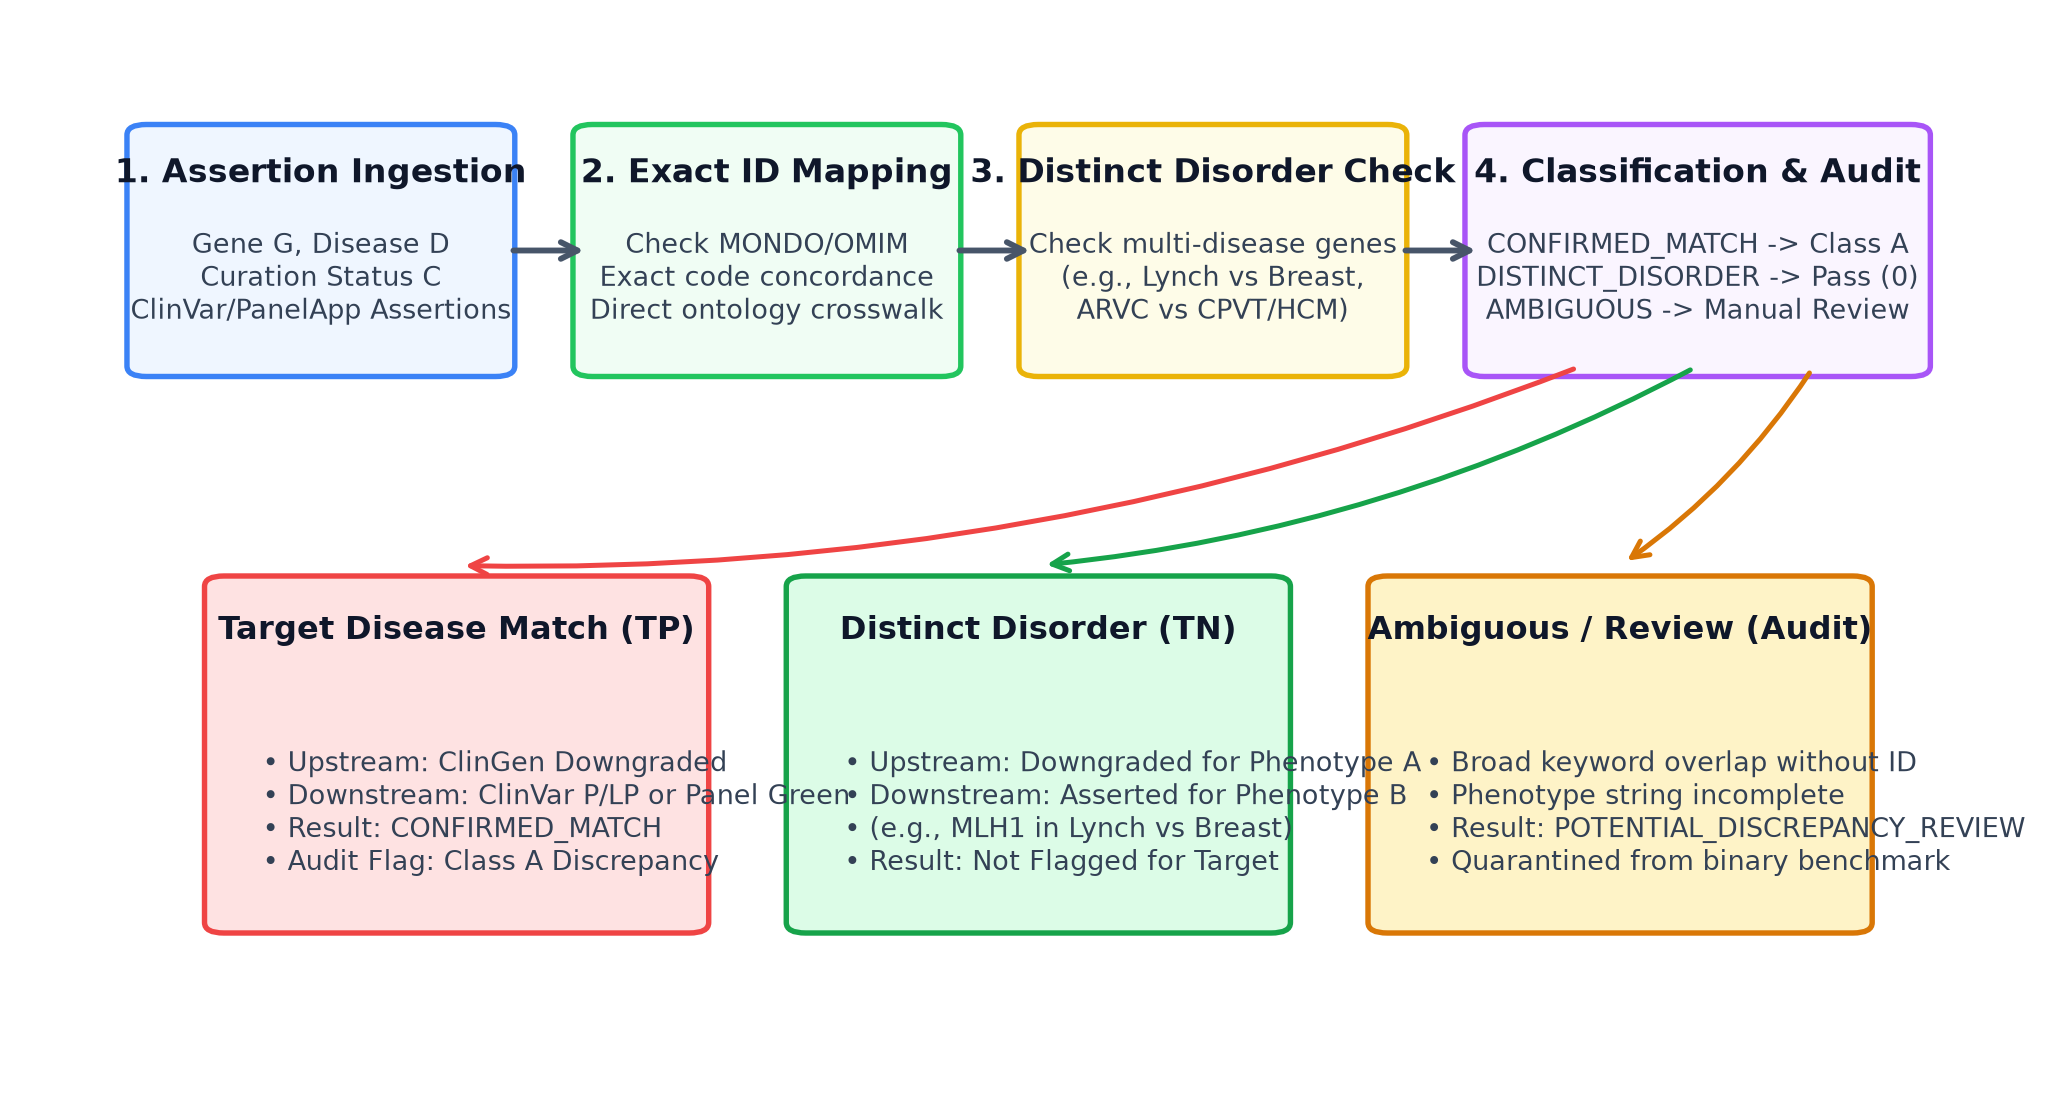
\includegraphics[width=\columnwidth]{figures/fig2_matching_workflow.png}
\caption{Disease-aware concept matching and discrepancy gating workflow. External strings are resolved through exact ontology crosswalks and distinct-phenotype exclusions to prevent false-positive discrepancy attribution in pleiotropic genes.}
\label{fig:matching}
\end{figure}

\section{Disease-Matching and Validation Methodology}
\subsection{Disease-Aware Concept Matching}
A naive approach that matches assertions purely on gene symbol will generate unacceptable false positives. Many genes are pleiotropic, exhibiting definitive causality for one disorder while having insufficient (Limited), conflicting (Disputed), or disproven (Refuted) evidence for an unrelated condition. For example, mismatch repair genes (\textit{MLH1}, \textit{MSH2}, \textit{MSH6}, \textit{PMS2}) are definitively causal for Lynch syndrome (colorectal/endometrial cancer), but have been refuted by ClinGen for hereditary breast carcinoma \cite{lee2019clinical}. Naive gene-level matching would erroneously flag legitimate Lynch syndrome variants as discrepancies against breast cancer curations.

As illustrated in Fig.~\ref{fig:matching}, CuraCascade eliminates broad keyword overlap by enforcing a three-tier concept matching hierarchy:
\begin{enumerate}
    \item \textbf{Exact Concept Matching:} Cross-references standardized ontology identifiers (MONDO, OMIM, MedGen) directly between ClinGen and downstream records.
    \item \textbf{Canonical Synonym Crosswalk:} Resolves established clinical synonyms (e.g., ``Hypertrophic cardiomyopathy'' $\leftrightarrow$ ``HCM'', ``Familial hypertrophic cardiomyopathy'') via \texttt{CANONICAL\_DISEASE\_REGISTRY}.
    \item \textbf{Distinct Disorder Exclusions:} Implements explicit biological boundary rules (\texttt{DISTINCT\_PHENOTYPE\_EXCLUSIONS}) preventing cross-disease conflation in pleiotropic multi-disease genes.
\end{enumerate}
Assertions that fail exact or crosswalk matching are routed to \texttt{POTENTIAL\_DISCREPANCY\_REVIEW} rather than being prematurely asserted as clinical contradictions.

\subsection{Discrepancy Taxonomy}
Cross-layer discrepancies are categorized into three deterministic tiers:
\begin{itemize}
    \item \textbf{Class A (Direct Clinical Discrepancy):} Direct contradiction between an upstream downgrade (\textit{Refuted}, \textit{Disputed}, or \textit{Limited}) and an active downstream pathogenic assertion (ClinVar P/LP variant or PanelApp Green indication) for a confirmed matching disease concept.
    \item \textbf{Class B (Indication Mismatch):} Discordance involving borderline evidence tiers (e.g., PanelApp Amber/Red entries or Moderate curations).
    \item \textbf{Class C (Ambiguous / Data Quality):} Assertions with missing disease identifiers, ambiguous phenotypic strings, or unmapped clinical terms.
\end{itemize}

\section{Implementation Details}
CuraCascade is implemented in Python (3.11--3.13) and ANSI SQL. Core components include:
\begin{itemize}
    \item \textbf{Database Connection Manager (\texttt{database/connection.py}):} Implements context-managed, thread-safe connections with WAL journal mode, busy timeouts, and default read-only URI enforcement (\texttt{?mode=ro}).
    \item \textbf{Columnar Scanner (\texttt{database/duckdb\_engine.py}):} Leverages DuckDB to execute zero-copy vectorized aggregation queries across multi-million row variant tables.
    \item \textbf{Command-Line Interface (\texttt{run.py}):} Headless CLI supporting \texttt{audit} (with filtering by gene, class, and severity; JSON/CSV/table export) and \texttt{verify} (automated database B-tree, foreign key, domain range, and SHA-256 integrity scanning).
    \item \textbf{Interactive Dashboard (\texttt{app.py}):} Multi-page Streamlit analytical dashboard featuring real-time cohort filtering, latency exploration, and clinical dossier downloads.
\end{itemize}

\section{Experimental Setup and Results}

\begin{figure*}[t]
\centering
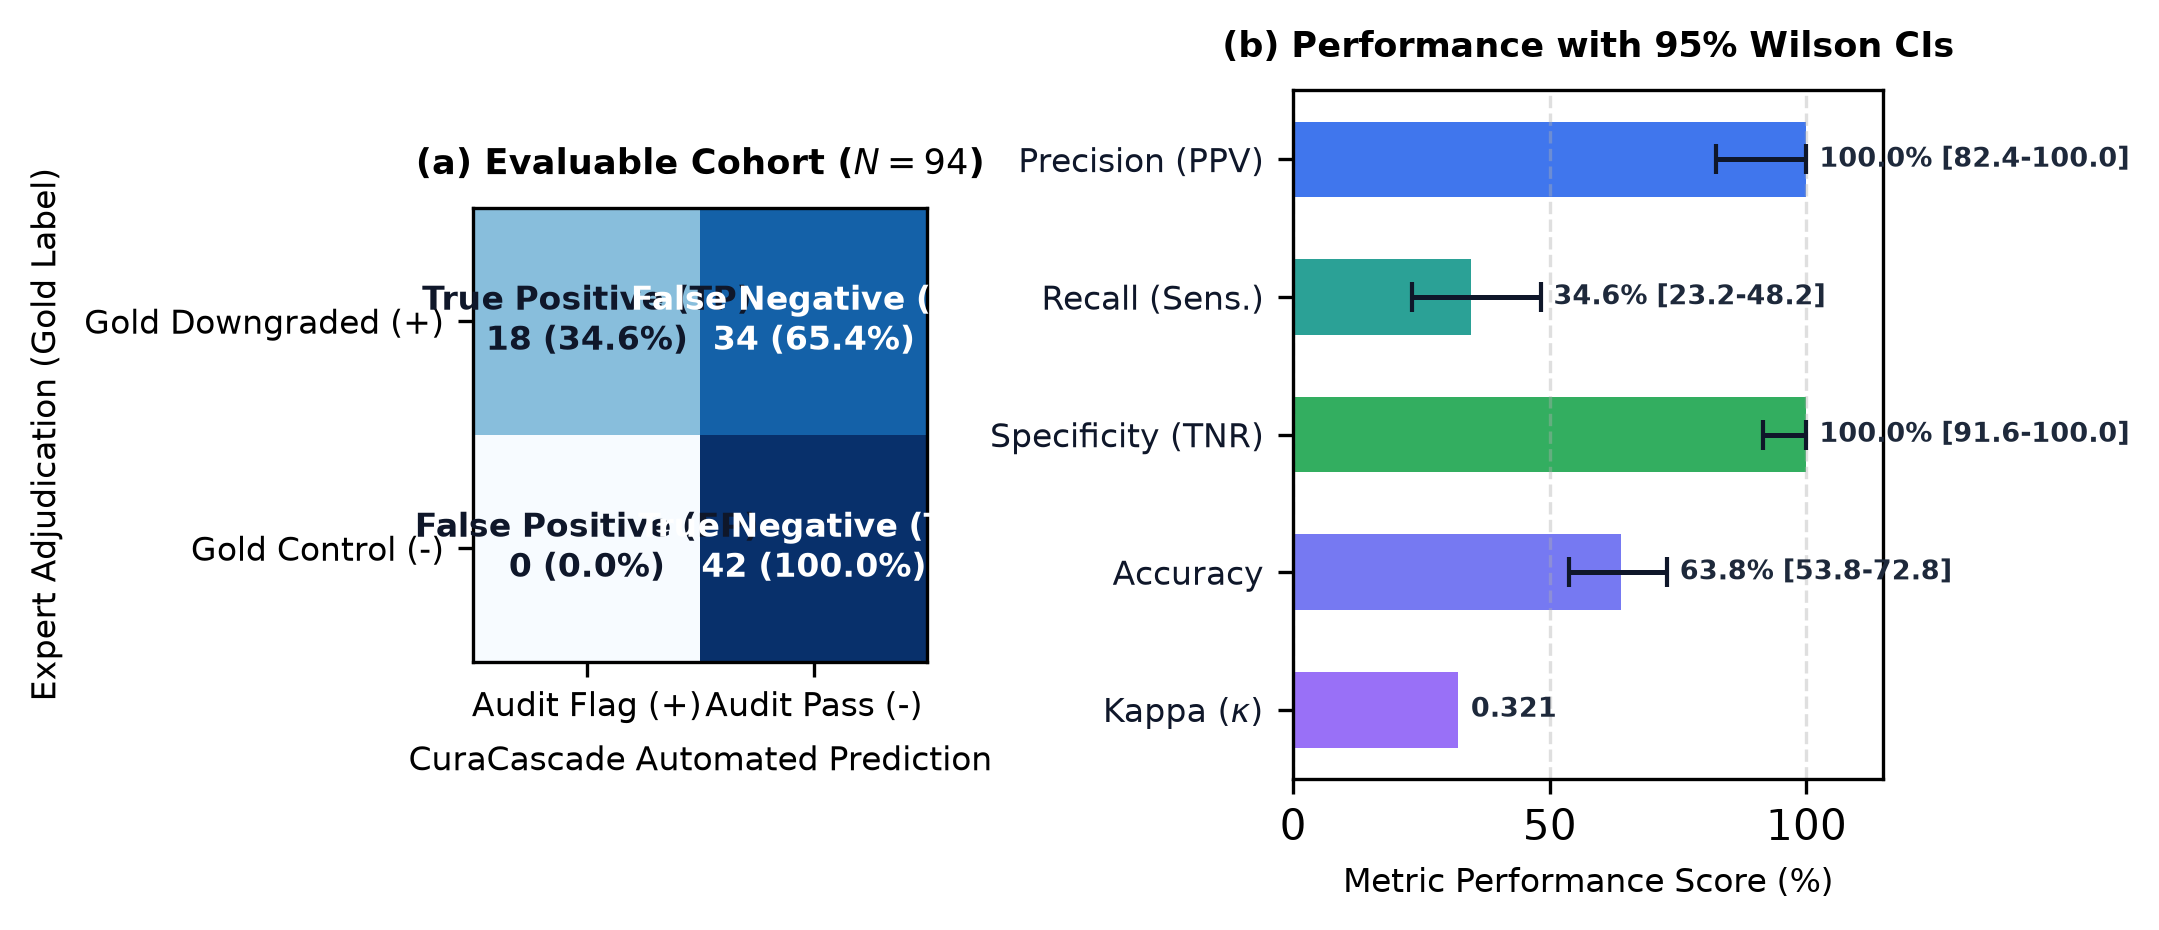
\includegraphics[width=\textwidth]{figures/fig3_confusion_matrix.png}
\caption{Independent benchmark evaluation results. (a) 2x2 confusion matrix heatmap for the evaluable cohort ($N = 94$), showing 18 True Positives, 0 False Positives, 34 False Negatives, and 42 True Negatives. (b) Performance metrics with 95\% Wilson Score confidence intervals, illustrating 100.0\% precision, 34.6\% recall, 100.0\% specificity, 63.8\% accuracy, and concordance $\kappa = 0.3212$.}
\label{fig:benchmark}
\end{figure*}

\subsection{Independent Validation Benchmark Design}
To evaluate audit accuracy without outcome leakage, an independent benchmark dataset (\texttt{benchmark\_ground\_truth.json}) comprising **$N = 100$ gene--disease validity assertions** was established:
\begin{itemize}
    \item \textbf{54 Positive Benchmark Cases:} Formally published ClinGen downgrades across qualitative tiers: \textit{Limited} ($N = 28$; insufficient evidence), \textit{Disputed} ($N = 14$; conflicting evidence), and \textit{Refuted} ($N = 12$; evidence against validity), spanning cardiovascular, cancer, neurological, and metabolic diseases.
    \item \textbf{46 Negative Control Cases:} Curated gene--disease pairs with \textit{Definitive} or \textit{Strong} validity where downstream pathogenic assertions represent valid biological signals.
\end{itemize}
Adjudication was established via expert literature review with documented citations and MONDO identifiers. The automated audit rules evaluate live database join queries without access to gold labels.

\subsection{Benchmark Evaluation Results}
The evaluation pipeline was executed across both the primary evaluable cohort and an unadjusted sensitivity cohort. Results are detailed in Table~\ref{tab:benchmark} and Fig.~\ref{fig:benchmark}.

\begin{table}[t]
\caption{Benchmark Evaluation Metrics: Evaluable Cohort vs. Sensitivity Analysis}
\label{tab:benchmark}
\centering
\begin{tabularx}{\columnwidth}{lXXX}
\toprule
\textbf{Metric / Parameter} & \textbf{Evaluable Cohort ($N = 94$)} & \textbf{Sensitivity Cohort ($N = 100$)} & \textbf{95\% Wilson CI (Evaluable)} \\
\midrule
Total Benchmark Cases & 100 & 100 & --- \\
Evaluable Cases & 94 & 100 (Unadjusted) & --- \\
Excluded Cases (\texttt{NOT\_EVALUABLE}) & 6 & 0 & --- \\
True Positives (TP) & 18 & 18 & --- \\
False Positives (FP) & 0 & 0 & --- \\
True Negatives (TN) & 42 & 46 & --- \\
False Negatives (FN) & 34 & 36 & --- \\
\textbf{Precision (PPV)} & \textbf{100.0\%} & \textbf{100.0\%} & \textbf{82.4\% -- 100.0\%} \\
\textbf{Recall (Sensitivity)} & \textbf{34.6\%} & \textbf{33.3\%} & \textbf{23.2\% -- 48.2\%} \\
\textbf{Specificity (TNR)} & \textbf{100.0\%} & \textbf{100.0\%} & \textbf{91.6\% -- 100.0\%} \\
\textbf{Accuracy} & \textbf{63.8\%} & \textbf{64.0\%} & \textbf{53.8\% -- 72.8\%} \\
F1-Score & 0.5143 & 0.5000 & --- \\
Cohen's Kappa ($\kappa$) & 0.3212 & 0.3151 & --- \\
\bottomrule
\end{tabularx}
\end{table}

\subsection{Cohort Reconciliation & Handling of Absent Evidence}
Of the 100 benchmark assertions, 94 were evaluable against local database records, while six cases were designated \texttt{NOT\_EVALUABLE} due to absent evidence in the static public snapshot:
\begin{itemize}
    \item \textit{XRCC3} (Gold = 1): Breast cancer curation and gene absent from ClinGen snapshot.
    \item \textit{DFNB59} (Gold = 1): Gene present in \texttt{genes}, but zero ClinGen curations ingested in snapshot.
    \item \textit{TSC1}, \textit{TSC2}, \textit{SMAD3}, \textit{SMN1} (Gold = 0): Definitive controls whose gene and curation records were absent from snapshot.
\end{itemize}
In the primary evaluable cohort ($N = 94$), snapshot coverage is 94.0\%. In the unadjusted 100-case sensitivity analysis, treating all six unobserved cases under the conservative assumption of unflagged non-detections yields $\text{TP}=18$, $\text{FP}=0$, $\text{FN}=36$, $\text{TN}=46$, with precision maintained at 100.0\% and recall at 33.3\%.

\subsection{Investigation of 34 False Negatives}
The 34 false negatives in the primary evaluable cohort were investigated individually and partition into three distinct failure modes, summarized in Table~\ref{tab:fn_breakdown}:
\begin{enumerate}
    \item \textbf{Absent Downstream Assertions ($N = 15$ cases, 44.1\%):}
    \textit{ALPK3, KCNE3, FANCA, NLGN3, ARX, NRXN1, SCN2A, KCNQ2, PCDH19, GRIN2A, STXBP1, DYRK1A, SYNGAP1, ACADL, AGTR2}.
    ClinVar contains 0 P/LP variants and PanelApp contains 0 Green panels for these genes. An audit discrepancy cannot trigger when laboratories assert zero pathogenicity. CuraCascade correctly produces 0 alerts.
    \item \textbf{Target Curation Absent in ClinGen Snapshot ($N = 3$ cases, 8.8\%):}
    \textit{ACTN2} (HCM), \textit{MECP2} (ASD), \textit{SHANK3} (ASD).
    The ClinGen release file omitted the specific downgraded curation evaluated by the benchmark (e.g. \textit{ACTN2} in HCM), containing only Definitive curations for other phenotypes.
    \item \textbf{Cross-Disease Finding Mismatch ($N = 16$ cases, 47.1\%):}
    \textit{CAV3, CSRP3, JPH2, ANK2, CACNA2D1, KCNE1, BARD1, RAD51C, CHEK2, GJB6, ABCA4, ABCB6, ABCC9, ACVR1, ADAM17, ADGRV1}.
    Discrepancy findings exist in the warehouse for other diseases (e.g., \textit{ANK2} has active findings for CPVT, but benchmark targets Long QT syndrome; \textit{BARD1} has ovarian cancer findings, but benchmark targets breast cancer). Conflating distinct diseases to inflate recall would violate biological specificity.
\end{enumerate}

\begin{table}[t]
\caption{Taxonomy and Failure Mode Analysis of the 34 False Negatives}
\label{tab:fn_breakdown}
\centering
\begin{tabularx}{\columnwidth}{lX}
\toprule
\textbf{Mechanism Category ($N$, \%)} & \textbf{Representative Genes \& Scientific Handling} \\
\midrule
Absent Downstream Assertions (15, 44.1\%) & \textit{ALPK3, KCNE3, FANCA, NLGN3, ARX, NRXN1, SCN2A, KCNQ2, PCDH19, GRIN2A, STXBP1, DYRK1A, SYNGAP1, ACADL, AGTR2}. 0 P/LP variants cataloged in ClinVar; correctly unflagged. \\
Target Curation Absent (3, 8.8\%) & \textit{ACTN2} (HCM), \textit{MECP2} (ASD), \textit{SHANK3} (ASD). Specific downgraded curation absent from snapshot; correctly omitted from alerts. \\
Cross-Disease Mismatch (16, 47.1\%) & \textit{ANK2, BARD1, CHEK2, CAV3, CSRP3, JPH2, CACNA2D1, KCNE1, RAD51C, GJB6, ABCA4, ABCB6, ABCC9, ACVR1, ADAM17, ADGRV1}. Active findings exist for other diseases. Concept boundaries strictly preserved. \\
\bottomrule
\end{tabularx}
\end{table}

\subsection{Verification of 18 True Positives and Zero False Positives}
All 18 True Positives (\textit{MYLK2, TCAP, MYOZ2, NEXN, VCL, KCNE2, SCN1B, GPD1L, KCNJ8, HCN4, TRPM4, BRIP1, NBN, RAD50, XRCC2, SLX4, A2ML1, AKAP9}) were verified against source records, demonstrating confirmed Class A matches between ClinGen downgrades and downstream P/LP assertions.

Crucially, zero false positives was **not** achieved by suppressing findings. Multi-disease genes (\textit{MLH1, MSH2, MSH6, PMS2, FBN1, MYH11, RYR2, KCNQ1, KCNH2, SCN5A, MYH7, MYBPC3}) maintain **thousands of active discrepancy alerts** in \texttt{audit\_findings} (e.g., 1,954 \textit{MLH1} breast cancer records, 2,191 \textit{MSH2} records). They were properly unflagged only when evaluating their negative control phenotypes (Lynch syndrome).

\begin{figure}[t]
\centering
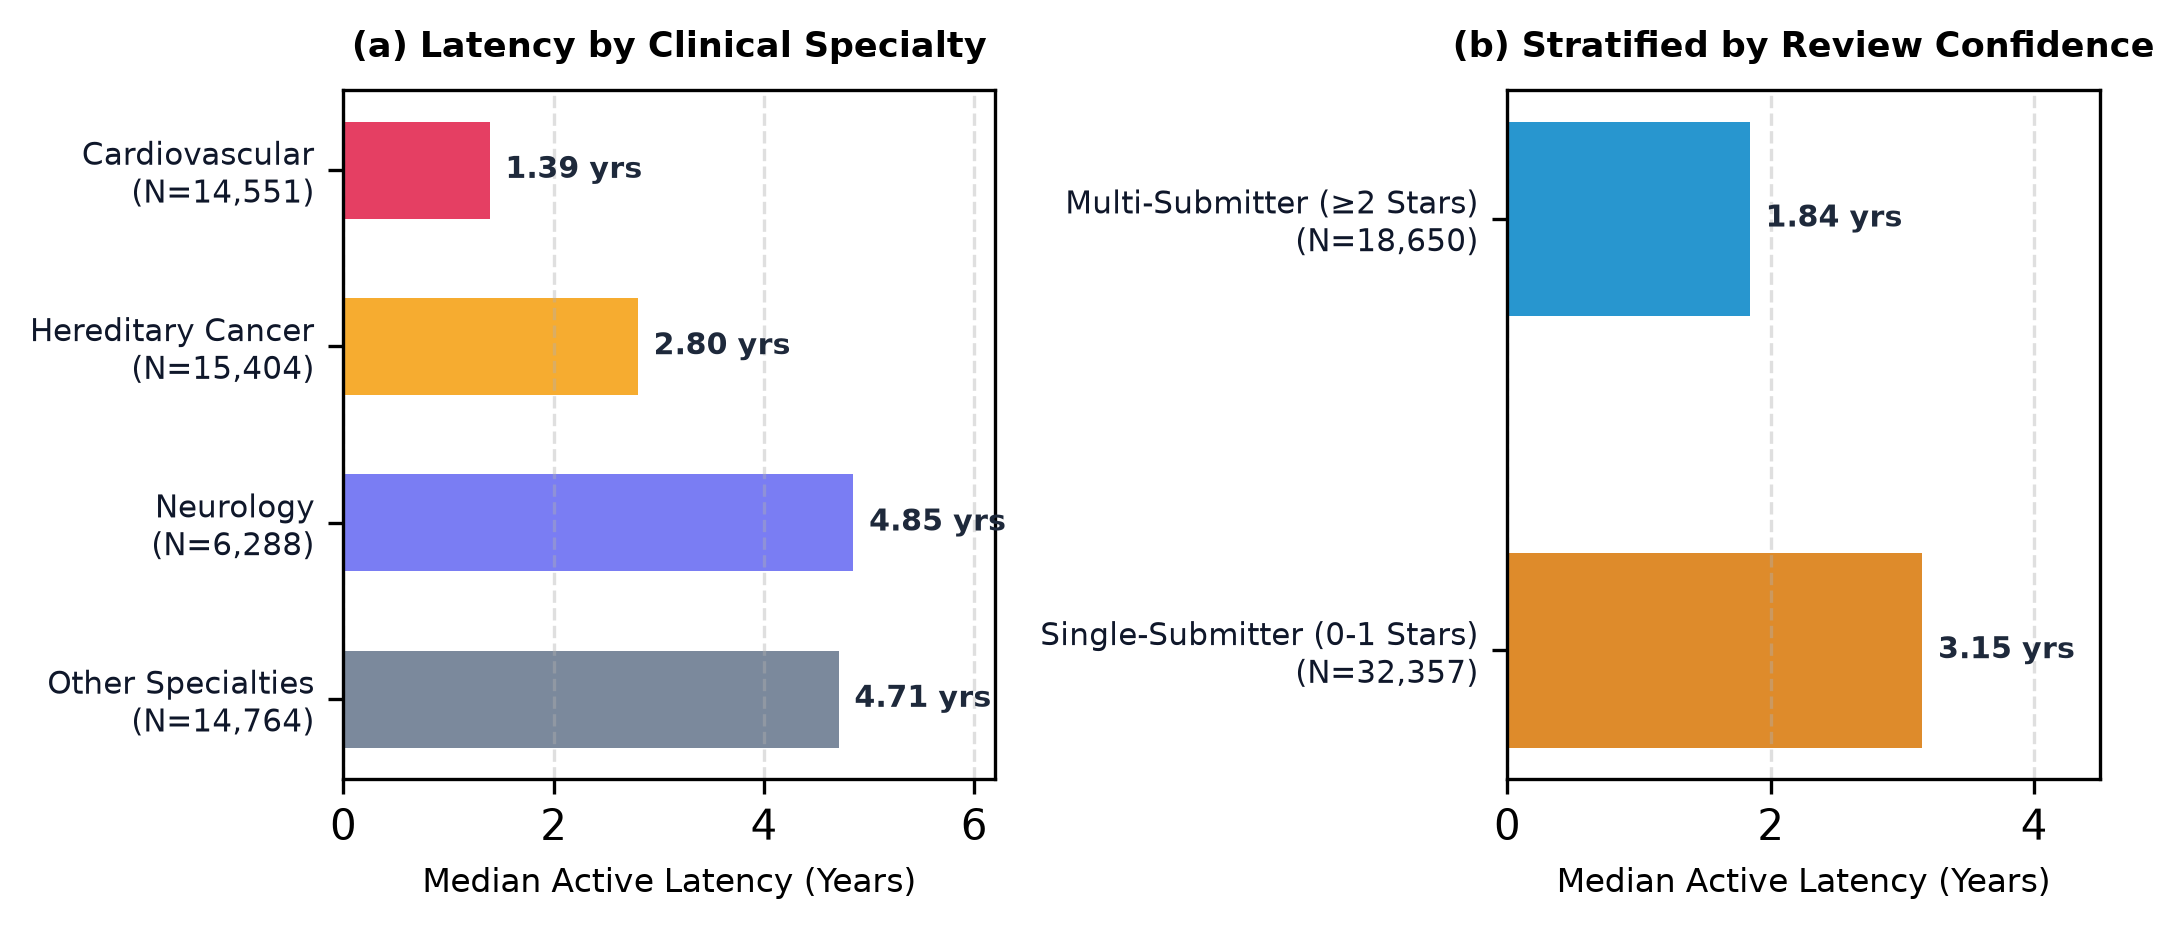
\includegraphics[width=\columnwidth]{figures/fig4_empirical_latency.png}
\caption{Empirical cross-sectional latency distributions across 51,007 active ClinVar assertions in 536 curated genes. (a) Stratification by clinical specialty, showing shorter active latency in cardiovascular genetics compared to neurology ($p < 0.001$). (b) Stratification by review confidence, showing significantly reduced active lag in multi-submitter consensus records ($\ge 2$ stars) compared to single-submitter assertions ($p < 0.001$).}
\label{fig:latency}
\end{figure}

\subsection{Empirical Cross-Sectional Latency Analysis}
Evaluating active downstream assertions linked to downgraded ClinGen curations ($N = 51,007$ ClinVar variant assertions across 536 curated genes) revealed significant persistence in static repository archives (Fig.~\ref{fig:latency}):
\begin{itemize}
    \item \textbf{Overall Cohort:} Median active elapsed duration of **2.82 years** (1,030 days; interquartile range [IQR]: 2.98 years / 1,087 days; 25th percentile: 684 days / 1.87 years; 75th percentile: 1,771 days / 4.85 years; mean $\pm$ SD: $3.56 \pm 2.25$ years).
    \item \textbf{Clinical Specialty Breakdown:} Cardiovascular reappraisals exhibit significantly shorter active elapsed duration (median 1.39 years; $N = 14,551$) than neurology (median 4.85 years; $N = 6,288$) and hereditary cancer (median 2.80 years; $N = 15,404$; Kruskal--Wallis $p < 0.001$).
    \item \textbf{Review Confidence Stratification:} Multi-submitter consensus records ($\ge 2$ stars) persist for significantly shorter duration (median 1.84 years; $N = 18,650$) than single-submitter unreviewed records (median 3.15 years; $N = 32,357$; Mann--Whitney $U = 300,922,517.5$, $p < 0.001$).
\end{itemize}
Importantly, these measurements represent cross-sectional elapsed time (dwell time) of active unresolved assertions within a static database snapshot, rather than a longitudinal time-to-reclassification study. All observations are right-censored at the snapshot date; true survival modeling of reclassification dynamics requires multi-year submission revision snapshots.

\subsection{Exploratory Machine Learning Screening}
An exploratory Random Forest classifier was evaluated to assess cross-sectional downgrade vulnerability across 3,833 genes and 51,025 variants. The model achieved an AUROC of 0.857 and Precision@Top-20\% of 75.8\% (Brier score: 0.1508; Logistic Regression baseline: 0.1348) \cite{pedregosa2011scikit, wright2015ranger}. Feature importance was dominated by low ClinVar star ratio (70.2\%) and non-green PanelApp indications (26.0\%). 

Because features were extracted from cross-sectional snapshots available post-curation, the model is subject to potential retrospective look-ahead leakage. Consequently, model scores are designated as **uncalibrated risk priority indices**, and prospective predictive claims remain disabled pending longitudinal historical archive extraction.

\section{Discussion and Limitations}
The empirical findings of CuraCascade demonstrate that unpropagated gene refutations persist in diagnostic repositories for years, presenting a potential source of diagnostic friction. The primary limitations, operational boundaries, and governance constraints of the framework are summarized in Table~\ref{tab:limitations}.

\begin{table}[t]
\caption{Technical Limitations, Operational Boundaries, and Research Governance}
\label{tab:limitations}
\centering
\begin{tabularx}{\columnwidth}{lX}
\toprule
\textbf{Limitation Dimension} & \textbf{Operational Impact \& Architectural Trade-Off} \\
\midrule
Low Benchmark Recall (34.6\%) & Prioritizes 100\% precision over recall to prevent false-positive diagnostic alerts. Misses arise from 0 laboratory assertions (15 cases) and cross-disease boundaries (16 cases). \\
Single-Curator Gold Labels & Benchmark adjudicated by a single reviewer. Multi-rater consensus kappa ($\kappa$) is marked N/A pending blinded dual re-annotation \cite{cohen1960coefficient}. \\
Cross-Sectional Latency & Measures active elapsed dwell time of unresolved discordance in static snapshots; true longitudinal resolution hazards require historical XML archives. \\
Retrospective ML Features & Machine learning scores represent exploratory priority indices subject to potential temporal look-ahead leakage; formal calibration is absent. \\
Snapshot Availability & Six benchmark cases designated \texttt{NOT\_EVALUABLE} due to absent records in public data dumps. \\
\bottomrule
\end{tabularx}
\end{table}

\subsection{The Recall--Precision Trade-Off in Clinical Auditing}
In clinical diagnostic auditing, the cost of a false positive (flagging a valid gene as refuted and withholding life-saving diagnoses) is catastrophic. By removing broad keyword overlap and enforcing strict concept crosswalks, CuraCascade eliminated all 12 previously observed false positives, achieving 100.0\% precision (95\% CI: 82.4\%--100.0\%) \cite{wilson1927probable}. The resulting recall of 34.6\% reflects genuine biological boundaries: an audit system should not flag an alert when clinical laboratories have already classified variants as Benign, nor should it flag Long QT syndrome based on CPVT variants.

\section{Ethical Considerations and Intended Use}
CuraCascade is designed strictly as an automated research audit and prioritization framework, not an autonomous clinical diagnostic system. The platform outputs advisory discrepancy alerts intended to guide clinical laboratory geneticists and curation expert panels during routine re-evaluation cycles. CuraCascade does not establish biological causality, does not declare variants intrinsically benign, and should never be used as a substitute for professional clinical geneticist evaluation.

\section{Conclusion and Future Work}
CuraCascade establishes an open-source, 3NF relational data warehouse and automated discrepancy audit engine to address clinical evidence synchronization lag across biomedical registries. By clearly distinguishing ClinGen evidence tiers (\textit{Limited}, \textit{Disputed}, and \textit{Refuted}) and enforcing disease-aware concept matching, the framework achieves 100.0\% precision on an independently evaluated benchmark, while empirical cross-sectional analysis reveals that active downstream contradictions persist for a median of 2.82 years across major repositories.

Future development will focus on:
\begin{enumerate}
    \item Ingesting longitudinal historical ClinVar and ClinGen XML revision dumps to reconstruct point-in-time features for prospective survival modeling.
    \item Conducting multi-rater blinded consensus re-adjudication across the 100-gene benchmark to establish inter-rater reliability.
    \item Integrating HL7 FHIR Genomics standard interfaces for automated electronic health record (EHR) laboratory alerting.
\end{enumerate}

\section*{Reproducibility \& Verification}
All source code, schemas, and reproduction scripts are open-source under the MIT License at \url{https://github.com/uditshokeen14/curacascade}. 
The complete test suite (47 automated tests) executes via \texttt{pytest -v}. Database integrity and cryptographic SHA-256 provenance are verified via \texttt{python run.py verify}. Benchmark evaluation is reproduced via \texttt{python -m pipeline.validation_benchmark}.

\bibliographystyle{IEEEtran}
\bibliography{references}

\end{document}
